\documentclass{article}
\usepackage[english]{babel}
\usepackage[utf8]{inputenc}
\usepackage{xspace}
\usepackage{graphicx,graphics} 
\usepackage{color}
\usepackage{amsmath}
\usepackage{amsfonts}
\usepackage{amssymb}
\usepackage{amsthm}
\usepackage{algorithm}
\usepackage{algorithmic}
\usepackage{longtable}
\usepackage{complexity}

\newcommand\rmatching{assignment\xspace}
\newcommand\mdelay{$\cal M$-delay\xspace}
\newcommand\matchedgraph{{\bf matched graph}}
\begin{document}


\graphicspath{{figures/}}
\newtheorem{rem}{Remarque}
\newtheorem{proposition}{Proposition}
\newtheorem{theorem}{Theorem}
\newtheorem{fact}{Fact}
\newtheorem{lemma}[theorem]{Lemma}
\newtheorem{definition}{Definition}
\newtheorem{corollary}{Corollary}

\title{Graph algorithm for deterministic routing to ensure latence in cloud RAN networks}

\newcommand{\todo}[1]{}
\renewcommand{\todo}[1]{{\color{red} TODO: {#1}}}
 
\author{MG, DB, CC, OM, YS}

  % ?

\maketitle

 
\section{Introduction}

\todo{A REPRENDRE POUR LA JUSTIFICTION RESEAU AVEC LE DETERMINISTIC ROUTING (OM?) ET INSERER LA PROBLMATIQUE GRAPHE (DB)}
 In this article, we will work on latency constraints in fronthaul.
Thus, this type of architecture confronts the problem of controlling 
the latency in the transfer process.  Low latency is considered critical for the 5G, in particular for the deployment of the C-RAN approach 
(allowing time constraints like HARQ to be fulfilled over non dedicated networks), or to reach E2E expected latency from 1 to 10ms 
(depending on targeted services). One specificity in the C-RAN context is not only the latency constraint, but also the periodicity of 
the data transfer between RRH and BBU.  New scheduling and routing paradigms and new technologies have to be considered to  guarantee 
delay constrained periodic data transfers. Dynamical optical bypass and dynamical management of the emission should be considered to
guarantee latency constraints. This is why this study is a contribution to the ANR project N-Green.

N-GREEN proposes a new type of switching/routing node and a specific network architecture exploiting WDM packets thanks to a new generation of optical add/drop multiplexers (WSADM: WDM slotted add/drop multiplexer). These packets having a fixed duration close to $1\mu $s are transported in a transparent way, to better exploit the switching matrix of the node; their headers will be transported over one dedicated wavelength at a lower bit rate, to reduce the physical constraints of the electronic processing and scheduler.

 Thus, this subject targets new scheduling and routing paradigms to solve this periodic and delay constrained data transfer.
 Indeed, one of the most promising approaches relies on the concept of Deterministic Networking (DN) such that one get rid of
 statistical multiplexing. The traditional queue managements are replaced by time based forwarding. Solutions for Deterministic 
 Networking are under standardization in IEEE 802.1 TSN group, as well at IETF DetNet working group.  To make DN working over a
 network composed of several nodes, it is required to manage the time at which the packets of deterministic paths are crossing each nodes. 

Considering a graph, modeling the network topology, and a set of routes from source nodes (modeling connections to the BBU) and destination 
nodes (modeling the RRH) in this graph, the purpose is to select, for each destination node a route from one source node to it and a periodic 
routing scheme allowing to periodically sent a packet to each base station without congestion conflicts between all such packets and to insure a minimum latency. In a slotted time model, the aim is here to minimize the duration of the period, with a constraint of the maximum length of routes to be
selected. Even if the selected set of routes is given this optimization problem has been shown to be  \NP-hard. From an algorithmic point of view,
the purpose of this project is first, to study the complexity and the approximability of this problem when the length of the routes is small
(which corresponds to realistic cases), and secondly, to propose and implement some heuristics to solve this problem on realistic topologies.


The major difficulty of this problem is the periodicity of the process. Indeed, a deterministic sending for the messages
between each pair BBU/RRH must not collide with the other messages sent by the others BBU/RRH in the same period, but also in the previous
and following periods. This problem may look like wormhole problem \cite{cole1996benefit}, very popular few years ago, but here, we want to minimize the time lost in buffers and not just avoid the deadlock, and the wormhole does not treat about the periodicity.

\subsection*{Related works}
\todo{IL FAUT REPARTIR DE CE QUI EST DANS LE MEMOIRE DE MAEL, PLUS LES ARTICLES D'ORDONNANCMENT DE TRAINS. JE (DB) M'EN CHARGE.}
\section{Model and problem description}
\subsection{Definitions}
We consider a symmetric directed graph $G=(V,A)$ modeling a slotted network. Each arc  $(u,v)$ in $A$ is characterized by an integer delay $Dl(u,v) \geq 1$ representing the number of slots from $u$ to $v$ on this arc. Note that for any arc $(u,v)$, $DL(u,v)=DL(v,u)$.

A route $r$ in $G$ is a sequence of consecutive arcs $a_0, \ldots , a_{k-1}$, with $a_i=(u_i,u_{i+1}) \in A$.  The {\em latency} of a vertex $u_i$ in $r$, with $i \geq 1$, is defined by $$\lambda(u_i,r)= \sum\limits_{0 \leq j <i} Dl(a_j)$$ We also define $\lambda(u_0,r)=0$.
The latency of the route $r$ is defined by $\lambda (r)= \lambda (u_k,r)$.  A routing function $\cal R$ in $G$ associates a route from $u$ to $v$ for any couple of different vertices $<u,v>$ in $G$.\\

Let $\cal C$ be an {assignment} in $G$, i.e., set of couples of different vertices of $G$. We denote by $\cal R_{\cal C}$ the set of routes ${\cal R}(u,v)$ for any $<u,v>$ in $\cal C$. 

Consider now a positive integer $P$ called {\bf period}. A {\bf $P$-periodic affectation} of $\cal C$ in $(G,{\cal R})$ consists in a set  ${\cal M}=(m_0, \ldots ,m_{c-1})$
of $c$ integers that we call {\bf offset}, with $c$ the cardinal of $\cal C$. Indeed, time is consider as consecutive periods of $P$ slots each and the number $m_i$ represents the first slot number used by the route $r_i \in {\cal R}_{\cal C}$ at its source.
We define the first time slot at which a message reaches any vertex $v$ in this route by $$t(v,r_i) = m_i+\lambda(v,r_i) \mod P.$$

Let us call $[t(v,r_i)]$ the values of the time slots used by a route $r_i$ in such a vertex $v$. 
Those values are forming a continuous set of values starting at $t(v,r_i) \mod P$ and ending at $t(v,r_i) + \tau \mod P$. A $P$-periodic affectation must have no {\bf collision} between two routes in ${\cal R}_{\cal C}$, that is $\forall r_i, r_j \in {\cal R}_{\cal C}, i \ne j$, with $\tau$ the size (in number of consecutive slots) of each message that must be periodically sent on each route of ${\cal R}_{\cal C}$,
we have $$[t(u,r_i)] \cap [t(u,r_j)] = \emptyset .$$

The main theoretical problem we have to deal with in this context is the following.\\

\noindent {\bf Problem  Periodic Routes Assignment (PRA)} 

\noindent {\bf Input:} graph $G=(V,A)$, set $\cal C$ of couples of vertices, routing function $\cal R$, integer $P$.

\noindent {\bf Question:} does there exist a $P$-periodic affectation of $\cal C$ in $(G,{\cal R})$?

We deal in next section with complexity of Problem PRA.\\

 \begin{figure}[H]
\label{could-ran}
\begin{center}
% \begin{tabular}{cc}
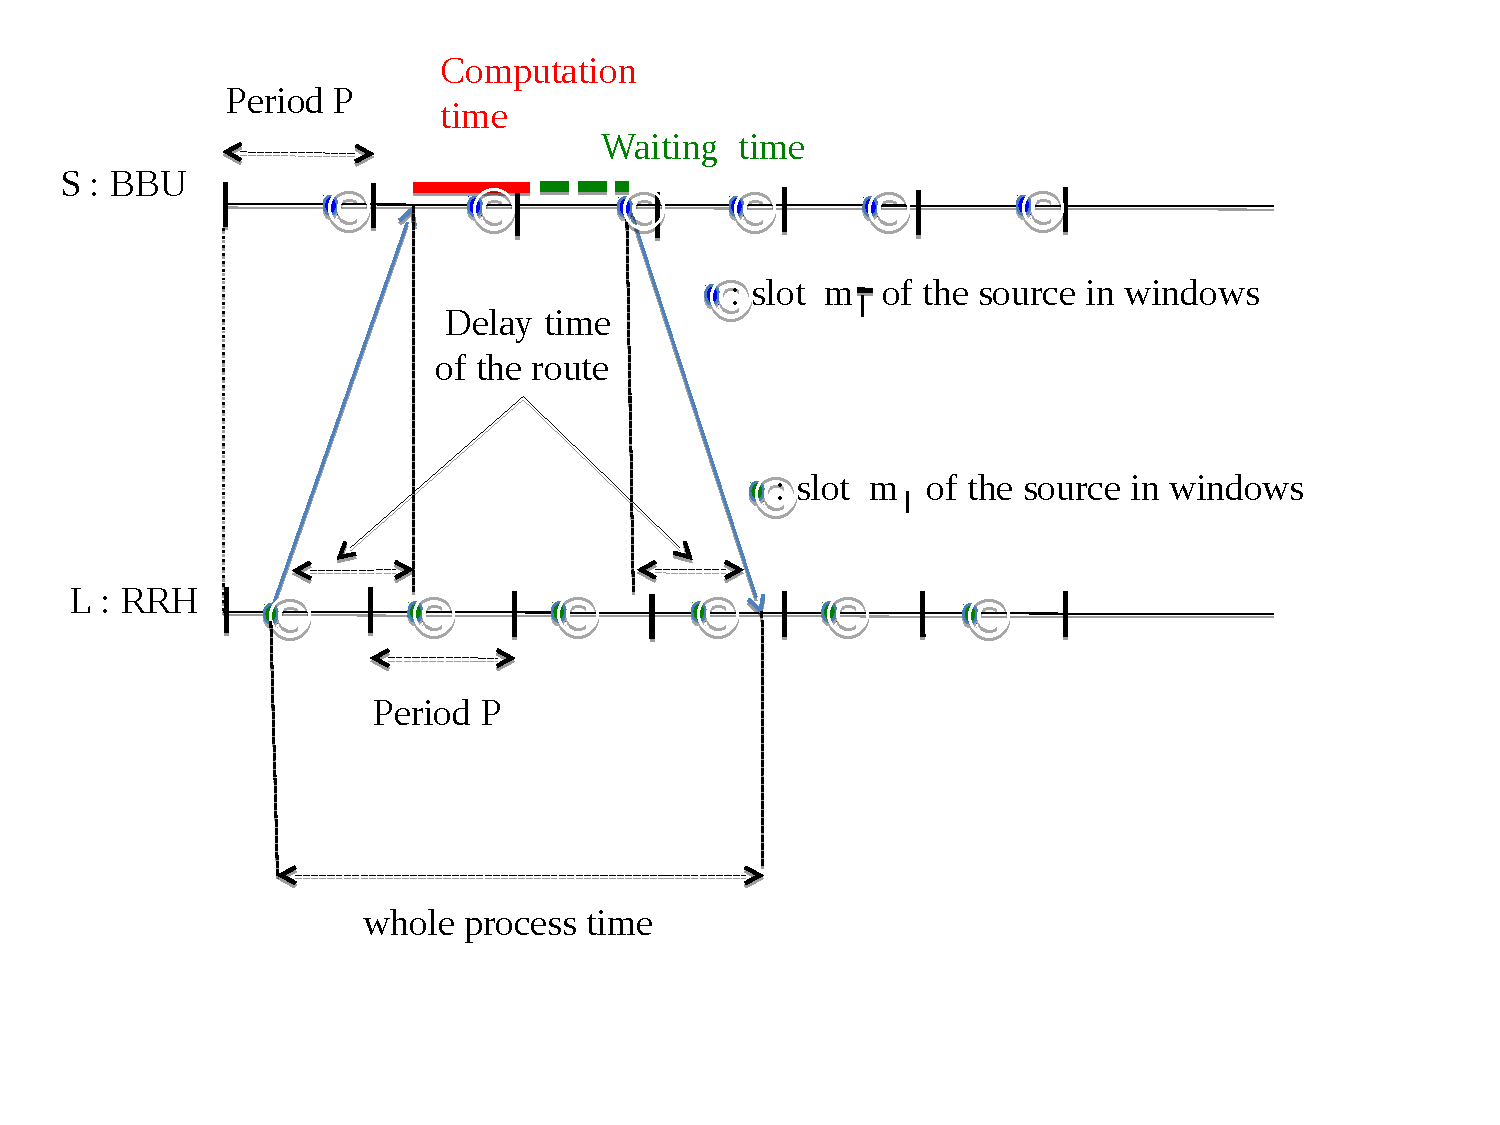
\includegraphics[scale=0.5]{Total-latence.pdf}
\caption{Complete process for a leaf in $L$.}
\end{center}
\end{figure}
%\end{tabular}\newline

In the context of cloud-RAN applications, we consider here in digraph $G=(V,A)$ modeling the target network two disjoint subsets of vertices $S$ and $L$, where $S$ is the set of BBU and $L$ is the set of RRH. We consider a {\bf matching} defined as an application $\rho:S\rightarrow L$. We consider a $P$-periodic affectation $\cal M$, associating respectively integers $m_l$ and $m_{\overline l}$ to couples $(l,\rho(l))$ and $(\rho(l),l)$ for all $l \in L$. The process realized periodically (i.e. initiated in each window of size $P$) for each leaf $l \in L$ is the following one (see Figure \ref{cloud-ran}). First, a message of $\tau$ slots is sent from $l$ to $\rho(l)$ on ${\cal R}(l,\rho(l))$ at slot $m_l$ in the current window. After receiving this message, $\rho(l)$ computes it during a time equal to $\theta$ slots. Then, a message of $\tau$ slots containing the computed result is sent back from $\rho(l)$ to $l$ on ${\cal R}(\rho(l),l)$, at the first occurrence of  step $m_{\overline l}$ in a window (i.e., in the current window at the end of computation or the next one). We denote by $\omega(l)$ the {\bf waiting time}of $l$, i.e.,  the number of slots between the end of the computation time in $\rho(l)$ and the first occurrence of  step $m_{\overline l}$ in a window. Thus, the whole proccess time for $l$ is equal to
$$
PT(l)=\lambda({\cal R}(l,\rho(l)))+\theta+\omega(l)+\lambda({\cal R}(\rho(l),l)).
$$
  
Let us denote by ${\cal C}_{\rho}$ the set of couples $<l,\rho(l)>$ and $<\rho(l),l>$, for any $l \in L$. Consider a $P$-periodic affectation ${\cal M}$ of ${\cal C}_{\rho}$ in $(G,{\cal R})$. The maximum process time of ${\cal M}$ is equal to equal to $MT({\cal M})=\max\limits_{l \in L} PT(l)$. Thus, we have to deal with the following problem.\\

\noindent {\bf Problem Periodic Assignment for Low Latency(PALL)} 

\noindent {\bf Input:}  a digraph $G$, a matching $\rho$ of a set $S$ into a set $L$ in $G$, a routing function $\cal R$, a period $P$, an integer $T_{max}$.

\noindent {\bf Question:} does there exist  a $P$-periodic affectation ${\cal M}$ of ${\cal C}_{\rho}$ in $(G,{\cal R})$ such that $MT({\cal M}) \leq T_{max}$?

The related optimisation problem we will focus on  consists in minimizing  $MT({\cal M})$. Note that in the context of cloud-RAN networks, we consider $P=1ms$, $\theta=2.6ms$ and $T_{max}$ must be less or equal to $3ms$.

 \section{Complexity results}
\subsection{Complexity of PRA and PALL}
Consider an instance of Problem PRA, i.e., a digraph $G=(V,A)$, an assignment $\cal C$, a routing function $\cal R$ and a period $P$. 
The \emph{conflict depth} of an assignment $\cal C$ is the  number of arcs crossed by at least two routes in ${\cal R}_{\cal C}$; in other words it is the number of potential conflicts between these routes. 
The \emph{load} of  an assignment is the maximal number of routes sharing a same arc (i.e., the congestion of this arc).
It is clear that a $P$-periodic affectation must satisfy that $P$ is larger or equal to the load.

We give two alternate proofs that PRA is $\NP$-complete.
The first one works for conflict depth $2$ and is minimal in this regards since we later prove that for conflict depth one,
it is easy to solve PRA. The second one reduces the problem to graph coloring and implies inapproximability. \\
 

 

 \begin{proposition}
Problem PRA is $\NP$-complete, for a routing with conflict depth two.
\end{proposition}
 \begin{proof}
  Let $H=(V,E)$ be a graph and $d$ its maximal degree. We want to determine whether $H$ is edge-colorable
  with $d$ or $d+1$ colors. We reduce this edge coloring problem to PRA. We define  from $H$ an instance $G,{\cal C}, {\cal R}, P$ as follows. For each 
  $v \in V$ there are two vertices in $G$  connected by an arc $(v_1,v_2)$ and none of these arcs are incident. The delay of these arcs is equal to $1$.
  The set $\cal C$ is made of couples of vertices $<s_{u,v}, l_{u,v}>$ for each edge $[u,v]$ in $H$ and the routes associated is ${\cal R} =s_{u,v},u_1,u_2,v_1,v_2,l_{u,v}$.  The delays of arcs $(s_{u,v},u_1)$ and $(v_2,l_{u,v})$ are equal to $d(d+1)-1$.  
    
  Let $\phi$ be an edge coloring with $k$ colors of $H$. We can build a $k$-periodic affectation of $\cal C$ in $(G,{\cal R})$
  by assigning to the source $s_{u,v}$ of each route an offset  of $\phi(s_{u,v})$. Indeed, 
  if two routes $r_1$ and $r_2$ in ${\cal R}_{\cal C}$ share the same edge, say $(v_1,v_2)$ then they represent two edges $e_1$ and $e_2$ of $H$ incident  
  to the vertex $v$. Therefore $\lambda(v_1,r_1) = \phi(e_1) \mod k$ because the delays of the edges before $v_1$ sum to $d(d+1)$ or 
  $2(d(d+1))$ which are equal to $0$ modulo $k$ since $k=d$ or $k=d+1$. Thus $\lambda(v_1,r_1) - \lambda(v_1,r_2) \mod k = \phi(e_1) - \phi(e_2) \mod k$
  and $\lambda(v_1,r_1) - \lambda(v_1,r_2) \mod k > 0$ since $\phi(e_1) \neq \phi(e_2) $.
  
  Now consider a $k$-periodic affectation of $\cal C$ in $(G,{\cal R})$ . For each $[u,v]$ in $H$, we define $\phi(u,v)$ to be the offset of the route
  beginning at $s_{u,v}$ in ${\cal R}_{\cal C}$. For the same reasons as in the last paragraph, $\phi$ is an edge coloring with $k$ colors.
  Therefore we have reduced edge coloring which is $\NP$-hard~\cite{holyer1981np} to PRA which concludes the proof. 
 \end{proof}
Solving Problem PALL implies to solve PRA for an assignment ${\cal C}_{\rho}$ defined on $S$ and $L$ (see Section 2). Thus, we have the following corollary :

\begin{corollary}
Problem PALL is NP-Hard.
\end{corollary}

As another corollary of the previous proposition,  given $G$, $\cal R$, $P$ and two disjoint subsets $S$ and $L$ in $G$, the problem of  knowing if there is a matching $\rho$  from $L$ in $S$ such that the answer to problem PRA for instance $G,{\cal C_{\rho}},{\cal R}, P$ is  $\NP$-hard since checking a potential feasible solution for this problem implies to solve PRA.\\

\todo{SOMMES NOUS SURS DE CES COROLLAIRES (YS et CC)????}


Consider now MIN-PRA as the minimisation problem related to PRA, consisting in minimizing the peril $P$.

\begin{theorem}
 Problem MIN-PRA cannot be approximate within a factor $n^{1-o(1)}$ unless $\P = \NP$ even when the load is two
 and $n$ is the number of vertices.
\end{theorem}

\begin{proof}
 We reduce PRA to graph coloring. Let $H$ be a graph instance of the $k$-coloring problem. 
 We define $G$ in the following way: for each vertex $v$ in $H$, there is a route $r_v$ in $G$.
 Two routes $r_v$ and $r_u$ share an arc if and only if $[u,v]$ is an edge in $H$; this arc is the only one shared by these two routes.   We put delays inbetween shared arcs in a route so that there is a delay $k$ between two such arcs. 
 
 As in the previous proof, a $k$-coloring of $H$ gives a $k$-periodic affectation in $G$
 and conversely. Therefore if we can approximate the minimum value of $P$  within a factor $f$,
 we could approximate the minimal number of colors needed to color a graph within a fator $f$, 
 by doing the previous reduction for all possible $k$. The proof follows from the hardness of approximability
 of finding a minimal coloring~\cite{zuckerman2006linear}.
\end{proof}


In particular, this reduction shows that even with small maximal load, the 
minimal period can be large.

 \begin{proposition}
The solution to MIN-PRA is either the load or the load plus one.
Moreover, a solution of  load plus one can be built in polynomial time.
\end{proposition}

\begin{proof}
 First we define an alerning path and how it characterizes an optimal solution of PRA.
 Let $v$ be a vertex of degree $d$ in the congestion graph (to be defined). We assume that the 
 coloring of the edges is optimal (to define in the case of a congestion graph). 
 The color $\alpha$ is not used in it neighborood. For every edge of color $\beta$ from this vertex
 we build an $\alpha - \beta$ path, that is a maximal path $u_0,u_1,\dots, u_l$ so that 
 $(u_0,u_1)$ is of color $\beta,\beta + \lambda(u_0,u_1)$, then $(u_1,u_2)$ is of color $\alpha + \lambda(u_0,u_1),\alpha +\lambda(u_0,u_2)$
 and so on (changer $\lambda$ car on ne suit pas des routes).
 
 A maximal $\alpha - \beta$ path must be a cycle or the coloring is not minimal.
\end{proof}
\todo{FINALISER CETTE DERNIERE PROPOSTION S'I Y A LIEU (YS ET CC)}

 \subsection{A polynomial case about PRA}
 
We now study special cases of problem MIN-PRA restricted to a subset.  First, we consider in this section instances $(G=(V,A),{\cal R}, {\cal C}_{\rho})$ of MIN-PRA in which the routing function is coherent.  A  routing function $\cal R$ is {\bf coherent} if and only if for any couples $<u,v>$ and $ <u',v'>$ of nodes in $V$ such that the two routes ${\cal R}(u,v)$ and ${\cal R}(u',v')$ cross two same vertices $x$ and $y$  in this same order, then the subroutes  from $x$ to $y$  in ${\cal R}(u,v)$ and ${\cal R}(u',v')$ are equal. As a consequence, for each node $u$ in $V$, the subgraph of $G$ induced by all the routes from $u$ to all the other nodes in $G$ is a tree.

Moreover, we also consider that for any pair of symmetric arcs $(u,v)$ and $v,u)$, routes ${\cal R}(u,v)$ and ${\cal R}(v,u)$ are also symmetric.

Finally, considering sets $S$ and $L$, set  ${\cal C}_{\rho}$ is obtained from an assignment $\rho$ of $S$ in $L$ such that  there are no common arcs for routes originating from different sources ($\rho$ is said {\bf source-free}).

\begin{proposition}
\label{DP-PRA}
Problem MIN-PRA restricted to instances $(G=(V,A),{\cal R}, {\cal C}_{\rho})$ within a coherent routing can be solved in linear time according to the size of $A$.
\end{proposition}

 The definition of source-free assignment ensures that an arc cannot belong to two routes in $\cal R$ originating from different sources in $S$. Moreover, the definition of a coherent routing  ensures that if two routes originate from the same source $x$, they share the same arcs from $x$ to a given vertex $y$ and cannot share an arc after. This means that $\forall (u,v) \in A$, the arcs $(u,v)$ with the highest load $l_{max} = max(load(u,v))$ are arcs $a_0^j$ sharing a common origin $u_0 \in S$ and a $P$-periodic affectation for those arcs is a $P$-periodic affectation for all the arcs in $A$.

A $P$-periodic affectation is such that routes on a same arc must be separated by a delay that is strictly superior to an integer $\delta \geq 0$. As a consequence, the minimum size of the period $P$ is equal to $l_{max} \times (\delta + 1)$. This means that that on the arc with the highest load, we can schedule the first route at the moment $m_k = 0$, the second route at a moment $m_{k'} = \delta + 1$ and so on for all $l_{max}$ routes. 

\begin{proposition}
\label{DP-NPA}
Giving $G$ and a coherent routing ${\cal R}$ ,finding a source-free assignment $\rho$ such that the  period solution to MIN-PRA is minimum over all such assignment can be done in linear time according to the size of $A$.
\end{proposition}

In any source-free assignment, the minimum size of $P$  is obtained by minimizing the highest load of the first arc of any route from a source to a leaf. As all sources in $S$ are connected to all sources vertices in $L$ by a route in $\cal R$, a simple load balancing allows to obtain a maximum load equal to  $max_{load} = \lceil \frac{\cal L}{|S|} \rceil$. Once the \rmatching is computed,  the minimum value of $P$ is thus equal to $max_{load} \times (\delta + 1)$.
 
%%%%%%%
We consider now instances $(G,{\cal R}, {\cal C}_{\rho})$ of MIN-PRA, called {\bf $1$-instances} in which the routing function is still coherent and $\rho$ is such that there exists one and only on arc crossed by at least $2$ routes originated from different sources.  
\begin{proposition}
\label{1-arc PRA}
Problem MIN-PRA restricted to $1$-instances can be solved in linear time according to the size of $A$.
\end{proposition}

Let $(a,b)$be the arc in $G$ crossed by at least $2$ routes originated from different sources, and let $r(a,b)$ be the set of such routes.  
In order to have a $P$-periodic affectation, the period $P$ must be large enough for all arcs in $r(a,b)$, thus the minimal size of $P$ is $P= load(a,b) \times (\delta + 1)$. Moreover, this is also the minimum solution for $MIN-PRA$. If we consider that if there exists a $load(a_b)$-periodic affectation $m_i \in \cal M'$ of each route $r_i$ in $r(a,b)$ , then $m_j$ in $\cal M$ corresponding to $r_i$ is $m_j = m_i - \lambda(u_b) mod P$ . As the routing function is coherent, no two routes originating from a same source can use different routes to attain $(a,b)$ thus the $P$-periodic affectation is valid for any arc $(u,v) \in A$ if it is valid on $(a,b)$.

 
\section{Heuristic approaches to solve PALL}
\subsection{Network topologies}
We will especially focus on three symmetric digraph topologies corresponding to realistic cases  of  fronthaul network. In those kinds of networks, we can differentiate three kinds of
topologies. Each one of them correspond to a real configuration, depending of the distance between the BBU and the RRH.
\begin{enumerate}
 \item Topology 1: A basic network topology, composed of some base stations, represented by source nodes $S$, all connected to the same switch,
which will be a vertex, connected itself to another vertex, corresponding to a switch, connected to some leave nodes $L$ representing the RRH.
\item Topology 2: A network containing an optical ring, such that some sources nodes be connected to it anywhere, not intersecting themselves before the ring,
and some set of leave nodes are also connected at any point of the ring.
\item Topology 3: The general case: A DAG, on which we may restrict parameters as the degree or the number of vertices to represent graphs corresponding to realistic networks.
\end{enumerate}

 \begin{figure}[H]

\begin{center}
 
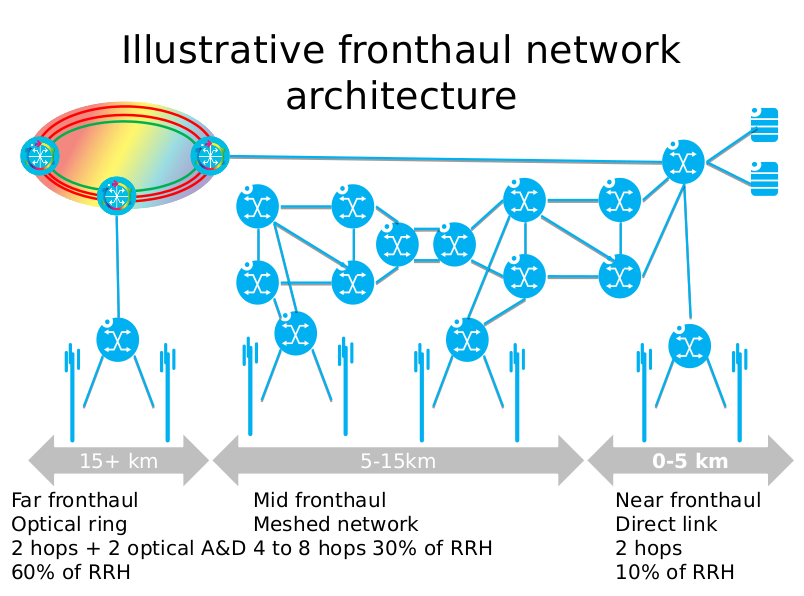
\includegraphics[scale=0.3]{fronthaul0.png}\\

\end{center}
\caption{From left to right: Topologies 2, 3 and 1 representing respectively the far, mid and near fronthaul.}
\end{figure}
 


\subsection{Algorithms}
...
\subsection{Performance evaluation}
...
\section{Conclusion}
...
\newpage
%%%%%%%%%%%%%%%%%%%%
%%%%%%%%%%%%%%%%%%%%%
%%%%%%%%%%%%%%%%%%%%%
\section{ANNEXE : MATERIEL SUPPLEMENTAIRE?}
\subsection{Coloring and $P$-periodic affectation}
We define two characteristic graphs associated to an assignment in $G$.

%\begin{definition}[Edge Conflict Graph]
%  The Edge Conflict Graph (ECG) of an \rmatching $\cal C$ in a digraph $G=(V,A)$ is the graph $G'=(V',E')$ such that 
 % a vertex of $V'$ is an arc of $A$ with a load greater than one. There is an edge between two vertices of $V'$
 % if and only if there is a route in ${\cal R}_{\cal C}$ which contains the two arcs of $A$ corresponding to the two vertices.
  
 % This graph can be oriented so that an edge is oriented as the route it represents and
 % we can associate as weight to this edge, the delay of the corresponding path.
%\end{definition}


\begin{definition}[Route Conflict Graph]
The Route Conflict Graph (RCG) of an \rmatching $\cal C$ in a digraph $G=(V,A)$ is the graph $G'=(V',E')$ where 
the vertices of $V'$ are the routes  in ${\cal R}_{\cal C}$ and there is an edges between two vertices in $V'$
corresponding to two routes in ${\cal R}_{\cal C}$ if and only if they share a same arc.

We fix an arbitrary ordering on the elements of $V'=\{v_1,\dots,v_n\}$.
We associate a weight to each edge $(v_i,v_j)$. Assume that $i < j$, 
and that the routes $r_i$ and $r_j$ in ${\cal R}_{\cal C}$ corresponding to $v_i$ and $v_j$ in $G'$ have $u$ as first common vertex.
Then the weight of $[v_i,v_j]$ is $\lambda(u,r_i) - \lambda(u,r_j)$.
\end{definition}
\todo{FAIRE LE LIEN ENTRE COLLORATION DU RCG ET P-PERIODIC AFFECTATION. NE FAUT-IL PAS INTRODUIRE LA TAILLE DE MESSAGE $T$ DANS LE SYSTEME D'INEQUATIONS? }
We define $\alpha(u,r_i,r_j) = | \lambda(u,r_i)-\lambda(u,r_j)|$. To the route conflict graph, we can associate a system of inequations representing the constraints that the 
$P$-periodic affectation must satisfy.

\begin{definition}[Conflict system]
 Let $G$ be a weighted RCG, we associate to each vertex $v_i$ of $G$ the variable $x_i$.
 The conflict system is the set of inequations $ x_i \neq x_j + w(e)$ for $i < j$ and $e=(v_i,v_j)$ edge of $G$.
\end{definition}

It is simple to see that the conflict system of a \rmatching has a solution modulo $P$ if and only if 
the \rmatching has a $P$-periodic affectation. This kind of system can be solved by SAT solver or CSP solver and those two methods will be investigated on practical instances.
\todo{Donner la formulation pour ces solvers et donner le résultat d'expérience dans une partie indépendante. 
Les comparer avec un solveur de notre cru avec quelques heuristiques simples.}

\begin{definition}[Additive coloring]
 Le $G$ be a weighted graph, we say that $G$ has an additive coloring with $p$ colors if and only if its associated
 conflict system has a solution over $\mathbb{Z} \diagup p\mathbb{Z}$. The minimal $p$ for which the system has a solution is the additive chromatic number of $G$ denoted by $\chi_{+}(G)$.
\end{definition}

Finding an optimal additive coloring is thus the same as solving our problem of finding a $P$-periodic affectation
and is at least as hard as finding an optimal coloring.  Because of the constraints on the edges, 
the additive chromatic number of a graph may be much larger than its chromatic number.
When the graph is a clique both additive and regular chromatic number may be the size of the graph.
However, we will now prove that for bipartite graphs the chromatic number is two while its additive 
chromatic number is arbitrary large.

We have the following values obtained by exhaustive search.

\todo{généraliser chi+ aux graphes sans poids en faisant un max ?}
\begin{fact}
 The values we list here are the maximal ones we obtain 
 by weighting bipartite graphs.
 \begin{enumerate}
  \item  $\chi_{+}(K_{2,2})= \chi_{+}(K_{3,3}) = 3$ with weight $0,1$
  \item $\chi_{+}(K_{3,4}) = \chi_{+}(K_{3,5}) =3$ 
  \item $\chi_{+}(K_{3,6}) = 4$ 
  \item  $\chi_{+}(K_{4,4})=\chi_{+}(K_{4,5})=\chi_{+}(K_{4,6})=4$
  \item $\chi_{+}(K_{5,5})= ?$
 \end{enumerate}
 \end{fact}

 A nice theoretical question would be to find the way to put weights
 on a bipartite graph so that its additive chromatic number is maximal. 
 My conjecture is that a $K_{l,l}$ can have an additive chromatic number in $O(l)$.
 The question is also interesting when we restrict the weights to $0,1$.
 
\begin{theorem}
 There is a weighting of $K_{l^2,\binom{l}{l^2}}$ such that 
 $\chi_{+}(K_{l^2,\binom{l}{l^2}}) > l$.
\end{theorem}

\begin{proof}
Let $V_1, V_2$ be the bipartition of the graph we build and let $|V_1| = l^2$. 
For all $S \subseteq V_1$ with $|S| = l$, we denote by $v_1,\dots,v_l$ its elements,
there is a single element $v_S$ in $V_2$ which is connected to exactly the elements of $S$
and such that the weight of $v_S,v_i$ is $i-1$. Because of this construction, $V_2$ is of size
$\binom{l}{l^2}$. Moreover for any additive coloring of the graph we have constructed,
a set of $l$ elements in $V_1$ cannot have all the same color. But by the extended pigeon principle, since there 
are $l^2$ elements in $V_1$ at least $l$ amongst them must have the same color. 
This prove that the graph we have built cannot have an additive coloring with $l$ colors.
\end{proof}

The theorem can be improved so that the number of colors is logarithmic in 
the size of the bipartite graph.

\begin{theorem}
 There is a weighting of $K_{l^2,\binom{l}{l^2}}$ such that 
 $\chi_{+}(K_{l^2,\binom{l}{l^2}}) > l$.
\end{theorem}

\begin{proof}
 Let $\mathcal{F}$ be a family of perfect  hash functions from $[l^2]$ to $[l]$. It means that for any 
 subset $S$ of size $l$ of $[l^2]$, there is an hash function $f \in \mathcal{F}$ such that $f_S$ is injective.
 The construction of the bipartite graph is similar to the previous proof. 
 Let $V_1, V_2$ be the bipartition of the graph we build and let $V_1 = \{v_1,\dots,v_{l^2}\}$. 
 For each function $f \in \mathcal{F}$ there is a vertex $v_f \in V_2$ and the weight of $(v_i,v_f)$ is $f(i)$.
 By \cite{schmidt1990spatial,alon1995color} there is a family of perfect hash functions of size $2^{O(l)}$ therefore $V_2$ is of size $2^{O(l)}$.
 Again by using the pigeon principle and the perfect property of the family of functions, we prove that no additive coloring with $l$ colors is possible.
\end{proof}

\todo{explain the removal of low degree vertices = kernelization + heuristic on the degree
Also implement it in the solver}

\todo{Comprendre la valeur sur d'autre familles de graphe, notemment celles qu'on peut rencontrer en pratique, par exemple petite tree width }


%%%%%%%%%%%%%%%%%%

\subsection{The disjoint paths NPAC-Problem : DP-NPAC}

In this problem, there is a delay constraint that must be satisfied by a \rmatching. This means that we must remove the routes in $r' \in \cal R$ where $\lambda(r') > K$.

\begin{proposition}
\label{DP-NPAC}
Problem DP-NPAC can be solved in polynomial time according to the size of $V$.
\end{proposition}

In a similar way to problem DP-PRA, the arcs with the highest load can only be the arcs $a_0^j$ sharing a common origin $u_i \in S$. In order to minimize the size of the period $P$, we have to find a \rmatching such that the maximum number $k_i$ of routes originating from a same source $u_i \in S$ is minimal. Having found this minimal value $k$, we face a problem equivalent to the DP-PRA problem.

In order to find a matching of vertices in $S$ with vertices in $L$ such that the maximum number of vertices in $L$ assigned to a vertex $s_i \in S$ is inferior or equal to $k$, we will transform our problem in a flow problem.

\subsubsection{Construction of a flow graph}

Let us consider an instance $I= (G=(V,A), S, L, \cal R, P, \delta, K$ and $M)$ of NPA where the routes in $\cal R$ are only those that respect the delay constraint $K$. We first construct a complete bipartite graph $G'=(V',A')$ where $V'$ is made of two sets of vertices : vertices $V'_1$ corresponding to $S$ and $V'_2$ corresponding to $ L$. $A'$ is made of all possible arcs from vertices $v'_1 \in V'_1$ to vertices $v'_2 \in V'_2$, with a capacity 1. We then add to $V'$ a source node $S'$ and a sink node $T'$. Finally we add to $A'$ all the arcs from $S'$ to each vertex $v'_1 \in V'_1$, with a capacity $k$  and all the arcs from each vertex $v'_2 \in V'_2$ to $T'$, with a capacity 1, where there is a route $\cal R$$(v'_1, v'_2)$. We have thus obtained a flow graph $G'$ whose size is polynomial in regards to the size of $G$. We will now compute the maximum flow in $G'$ in order to determine if its size is at least $\cal L$, in order to be able to connect all the leaves.

We can compute the size of a maximum flow in $G'$ in a polynomial time using a generic flow algorithm as Ford-Fulkerson (it will terminate as arcs capacity are rational numbers). In order to minimize the objective $k$, we can begin with a value $k$ = 1 and use a dichotomic approach to find the minimal value of $k$ for which a maximal flow of size $\cal L$ exists in $G'$. The maximum value of $k$ is $M$. If $k = M$ and the maximum flow value in $G' < \cal L$, then there is no valid \rmatching of $S$ in $L$.

The complexity of minimizing $k$ is thus $0(m^2n \times log_2 n)$ where $m = |A|$ and $n=|V|$. We obtain in the end a \rmatching minimizing the maximal number of routes originating from a single source $u_s \in S$ and we are faced with the DP-PRA problem for this instance.


\begin{figure}[!t]
\centering
includegraphics[scale=0.3]{DP-NPA.pdf}
\caption{Reduction of DPA-NPA into a flow problem}
\label{Modelling of DP-NPA Problem}
\end{figure}


\end{document}
%%%%%%%%%%%%%%%%%% 
  

  
\section{Real Network Topologies}

We consider 3 kinds of topologies corresponding to the different kinds of fronthaul networks: 
\begin{enumerate}
 \item Topology 1 : a basic network topology, composed of some base stations, represented by source nodes $S$, all connected to the same switch,
which will be a vertex, connected himself to another vertex, corresponding to a switch, connected to some leave nodes $L$ representing the Antennas.
\item Topology 2 : A network containing an optical ring, such that some sources nodes may join it anywhere, not intersecting themselves before the ring,
and some set of leave nodes are also leaving at any point of the ring.
\item Topology 3 : A ''random`` network, generated with some realistic properties (number of vertices, degree ...)
\end{enumerate}

\subsection{Topology 1}
\begin{center}
 
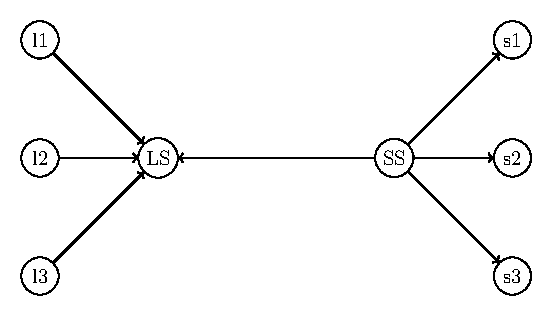
\includegraphics[scale=1]{Fig4.pdf}\\
Example of topology 1.
\end{center}

In this topology, there is 3 cases :
\begin{itemize}
 \item 1: When the weight of the links from source nodes are all equal. This is the closest case to the reality, but also the easier to solve.
 \item 2: When the weight of the leave nodes links are all equal .
 \item 3: When all the links have different weights.
\end{itemize}
The middle link can be represented without weight, because it is common to all the routes, so it can be simplified in calculations. 
Likewise, we do not consider $\theta$, the calculation time.

The first case is the easiest to solve. Indeed, it is obvious that if we schedule all messages following each others, we will obtain an optimal
$T_{max}$ : there is no waiting times on any routes.
Also, all the message will cross the first switch, without collisions, then 
they will not be another conflict point between all routes.

This solution is optimal because the messages will not wait on source nodes, so $\omega(r) = 0$, $\forall r \in \rho$. $T_{max}$ is
equal to the physical delay of the longer route, that we can not minimize.\\


Given this observation, one can try to solve a simpler problem for cases 2 and 3 : is it possible to find a two way trip
with all $w_i = 0$ ? 

It is always possible when the windows $P$ is large enough(for example: send all messages one by one, waiting the previous one to be back),
therefore the problem is to find the smallest windows such that it is possible.


The following example shows us that you can find a 2-way-trip affectation such that there is no waiting time, but it needs a greater time window P than a
solution with waiting times.

Consider the graph : 
\begin{center}
 
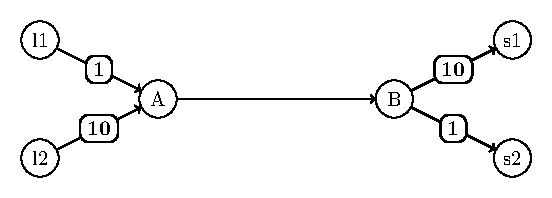
\includegraphics[scale=0.7]{Fig10.pdf}
\end{center}


Consider messages of 10 slots. If you search for a P-periodic affectation, without using waiting times, there are 2 choices : 
\begin{itemize}
 \item l1 is sent before l2 : the message from l1 will leave A after 11 slots.X is he minimal time slot in which l2 can emit. 
 To avoid collisions with the message from l1 in A,l2 must emit after 1 slot :  $X\ge1$.
 In the other way, the message from l1 will use B from time slot 21 to 30. The route from l2 is 12 units long from l2 to B. So, to avoid collisions with 
 the message from l1 in B $X+12 \ge 31 \rightarrow x\ge 19$. Then, by taking $X=19$, the time
 windows is at least 38 slots in A (corresponding to the transit time of the 2 messages and the time lost between those 2 transits).
 \item l2 is sent before l1: symmetrically the collision the collision occurs in node A if l1 emits before time 19. The time window in B is at least 38 too.
\end{itemize}

If we allow waiting times: there is an easy scheduling using only a 3 time slots windows : 
Sending message 1 at time 0, message 2 at time 1, so the messages will not cross A in the same time. to be sent back,
message 2 comes back immediately and is using B from slots 13 to 22,then message 1 is using B from slots 23 to 32, waiting 2 time slots at s1.

So the smaller time windows is 20, half smaller than best solution without waiting times.

\todo{temps de traje 22 contre 24 On peut utiliser l'exemple décrit en rajoutant un très long chemin de manière à ce que les 
waiting times ne changent pas la taille du plus long two way trip.}

Let us define a simplification of a matched graph. Ignore weights on arcs starting from leaves, and find a starting order without collisions 
(then to find the real values,add the corresponding delay to each routes). 
We obtain a graph in which we have a central node, and different routes going to each sources.
Such a graph is called a \emph{star}. A star is a non-oriented graph in which each edge between the central node $C$ and each source node $s_i$
has a weight $a_i$ (corresponding to the weight of the arc in $N$), where i is the number of the route in $\rho$. The r-matching $\rho$ is now
associating a route $r_i$ to a source node $s_i$.

\begin{center}
 
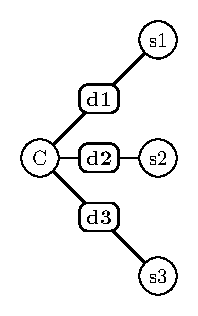
\includegraphics[scale=0.7]{Fig11.pdf}\\
example of a star for a matched graph with 3 routes
\end{center}


We can do this simplification of a matched graph N only if we search an affectation without waiting times : in this case, any solution
will be optimal, because the $T_{max}$ will be twice the delay of the longer route. So, a solution for a star, is a solution for a matched
graph, without waiting times. If waiting times are allowed, we are forced to consider the delay of the routes and this model is not
available anymore.

A \emph{star affectation} is a 2-way-trip affectation of the corresponding matched-graph $N$
in which there is no waiting time,$\omega(r) = 0 \,\forall\, r \,\in\, \rho$. 

In this simplified model, we have two parameters left: the begin offsets $o_i$ and the travel time of each routes $2a_i$.
A route may have no collisions with the others : $\forall$ i,j $\in \rho$, 
$$o_i \notin [b_i,...,b_i+T] \, and\, o_i+2a_i\notin [o_j+2a_j,...,o_j+2a_j+T].$$
T is the size of the message.


We define a new problem : 


\noindent {\bf Star affectation (SA)} 

\noindent {\bf Input:} a star s, integer $P$.

\noindent {\bf Question:} does there exist a star affectation of s in a period P.

\noindent {\bf Optimization :} minimizing P .\\

Solving this problem in P is finding the best solution for cases 2 and 3 of the topology 1.

We suggest the following algorithm to find a star affectation in which $d_0$ is the shortest route, and $d_{l-1}$ the longest one, 
l is the number of routes and T is the size of the messages :

\begin{algorithm}[H]
\caption{Star affectation from shortest to longest}
\begin{algorithmic}
\REQUIRE star s
\ENSURE star affectation in $P \le l*T + 2d_{l-1} - 2d_0$
\STATE $offset \leftarrow 0$
\FORALL{routes i in $\rho$ from the shortest to the longest }
\STATE $o_i \leftarrow offset$
\STATE $offset \leftarrow offset+T$
\ENDFOR

\end{algorithmic}
\end{algorithm}

The message using the shortest route is sent before the others, so it come back to the central node before the others.
Recursively, the second message is sent before the others, and also will be back before the other messages. 
Because the second message is sent T slots after the first message ($o_2 = o_1 + T$, where T is the size of the message), it come back after
the end of the message one : $o_1+ T + 2a_1 \le o_2 + 2a_2$ with $a_2 \ge a_1$.

The period given by this algorithm is P = 2$\lambda(r_{{\cal L}-1}$) + ${\cal L}$ * T - 2$\lambda(r_0)$, if routes $\{r_0,...,r_{{\cal L}-1}\}$ are ordered
from the shortest to the longest. 2$\lambda(r_0)$ is the first slot in which the first message is back, and 2$\lambda(r_{{\cal L}-1})$ is
the first slot in which the last message is back.${\cal L}$ * T is the time to transfer the messages from all routes.\\


We can also use a greedy algorithm, choosing the offset of each packet in turn so that there is no collision. We must chose an offset $o_i$ for each route $r_i$, so that no two routes have a collision on the central link the two times they use it.  We denote by $[o_i]_P$ the set of times $\{ t \mod P \mid o_i \geq t < o_i + T \}$ which are the time used by the route $r_i$ on the central link on its first use. There are no collision if for all $i\neq j$
 $[o_i]_P \cap [o_j]_P = \emptyset$. Moreover no two routes must have a collision on the way back, hence we must have for all $i\neq j$
 $[o_i + a_i]_P \cap [o_j + a_j]_P = \emptyset$.
 
One can prove that if $P$ is large enough with regard to $l$ and $T$, then there is always a two way trip
with waiting time $0$ with this algorithm.
 Assume $P \geq 4lT$, the algorithm works as follows. 
We cut the time windows of size $P$ into $2l$ slots of size $2T$ and we will asign one to each route.
A different slot is assigned to each route, where the offset is chosen inside the slot so that 
no collision on the first go in the central link is possible. If the slot chosen for the route $r_i$ is $[cT,(c+2)T]$,
then we set $o_i \in [cT,cT+1]$ so that $o_i + a_i \mod P = dT$. Assume that the offset of the first $i-1$ routes have been 
chosen in the previous way so that there is no collision. Since we have $P \geq 4lT$, we have at least $2l-i$ possible choices of offset without collision on the first use of the central link. Each of these choices uses a time slot of size $T$ on the way back on the central link. Since there are $i$ time slots used, and $i \leq l$, we have strictly more than $l$ possible choices and less than $l$ of them are forbidden, therefore there is a choice of offset with no collision. 
Since the algorithm works for all $i \leq l$, it finds a two way trip with waiting times $0$. 

\todo{On peutfaire mieux que $4lT$, avec une meilleure analyse ça doit juste gagner un tout petit peu, 
avec un meilleur algo de placement peut-on faire $3lT$ ou même $2lT$ ? Il doit être possible
de montrer qu'on ne peut pas faire mieux que $2lT$.} 



\begin{algorithm}[H]
\caption{start assignment greedy algorithm}
\begin{algorithmic}
\REQUIRE star s, window size $p$
\ENSURE star affectation in P<p 
\STATE $P1[p/2T]$ slots in first way period.
\STATE $P2[p/T]$ slots in back way period.
\FORALL{route i in $\rho$ }

\FORALL{slot j in P1}

\IF{P1[j] is free}

\STATE shift $\leftarrow$ T- 2$a_i \mod p$ 

\IF{P2[shift + 2Tj] is free}

\STATE $o_i \leftarrow 2Tj + shift$
\ENDIF

\ENDIF

\ENDFOR

\ENDFOR

\end{algorithmic}
\end{algorithm}

In this algorithm,for each route, search for a free time slot in P1,then set $o_i \in [cT,cT+1]$ so that $o_i + a_i \mod P = dT$.
If $[dT,(d+1)T]$ is free, and allow the route to use the time slot $[cT,cT+1]$ at the first use of middle link.\\

The following algorithm is a simplified way to find a star affectation

\begin{algorithm}[H]
\caption{start assignment greedy algorithm v2}
\begin{algorithmic}
\REQUIRE star s, window size $p$
\ENSURE star affectation in P<p 
\STATE $P1[p]$ slots in first way period.
\STATE $P2[p]$ slots in back way period.
\FORALL{route i in $\rho$ }

\FORALL{slot j in P1}

\IF{$[j,j+T]_P$ is free in P1}

\IF{$[j + 2r_j,j + 2r_j+T]_P$ is free in P2}

\STATE $o_i \leftarrow j$
\ENDIF

\ENDIF

\ENDFOR

\ENDFOR

\end{algorithmic}
\end{algorithm}

In this algorithm,for each route, search for the first free slot [j,j+T] in P1 such that the slot $[j + 2r_j,j + 2r_j+T]_P$ in P2 is free too,
then give the route the offset j(shifted by the distance from the leave to the first node).\\

Now, the waiting times are allowed, and try to solve PALL on topologie 1.
The following heuristic is suggested :

\begin{algorithm}[H]
\caption{Longest to shortest with waiting times}
\begin{algorithmic}
\REQUIRE Matched graph N, window size $P$, packed size T
\ENSURE 2way Trip affectation in P
\STATE offset $\leftarrow$ 0
\FORALL{route i in $\rho$ from the longest to the shortest }
\STATE  $m_i \leftarrow$ offset
\STATE offset $\leftarrow$ offset + T
\ENDFOR
\STATE offset $\leftarrow$ 0
\STATE take i such that $r_i$ is the first route to come back in sources node
\STATE $w_i \leftarrow $ offset;
\STATE offset $\leftarrow$ $a_i$ + T
\WHILE{there is a route which has no $w_i$}
\STATE take i such that $r_i$ is the longest route able to come back in source node before the last one has totally passed
\STATE $w_i \leftarrow $ offset - $a_i$;
\STATE offset $\leftarrow$ offset + T

\ENDWHILE

\end{algorithmic}
\end{algorithm}

The running of this algorithm is the following one :
\begin{itemize}
 \item 1 On leaves node, the messages are scheduled so that they are following each others, from the longest route to the shortest route.
 \item 2 On sources node, let the message able to come back first pass.
 \item 3 Once this message has passed, look at all the eligibles message able to be back at the sources node during the transit of the previous one.
 \item 4 Let the eligible message on the longest route transit in the node first after the previous one, possibly delayed by a little waiting time to avoid crossing.
 \item 5 delay the others with a waiting time.
 \item 6 while all the messages are not scheduled, get back to 3
\end{itemize}

This algorithm gives us solution with the minimum period possible : ${\cal L}$ x T. Indeed, all the messages are scheduled following each others on conflict node :
there is no wasted time between the transit of two messages.


For the case 1, this algorithm is similar to the obvious way to schedule the messages mentioned above. It gives optimal solution without increase 
the calculation time.

For the case 2, this algorithm gives optimal solutions: Indeed, in the manner we order messages, from leaves toward sources,
the messages are sent from the one using the longest route to the one using the shortest one. Number the routes in this order from 1 to ${\cal L-1}$.

We have $\forall \ i<j$, $r_i<r_j$.
The first message leaves the source switch at time 2$r_1+T$, the second message, can use it at the time 2$r_2+T$.
The second message waited $2r_1+T-2r_2+T = 2(r_1+r_2)$ to use the middle link. So, the second message leave the source switch at time
2$r_2+T + 2(r_1+r_2) = 2r_1 +T$.
Recursively, all messages will take $2r_1 +T$ slots for the Two Way Trip.
Consequently, for this case, the heuristic is optimal, because the longer route has no waiting time and no TwoWayTrip is longer than the longer route one.

For the case 3, after some simulations on values corresponding to reality $(P\simeq19500,T\simeq2500,l\simeq2000)$, good solutions are obtained. 

The average of solutions given by this heuristics gives solutions close to the average of $2*r_max$.

\todo{interessant de dire que la pire solution correspond souvent a celle trouvé par l'algo ? (sur ce genre de ''pire`` solutions, on ne peux pas
faire mieux.}
\todo{mettre l'exemple ou ca marche mal alors qu'en espacant un peu ca rentre tres bien}



% \section{Heuristics to solve PRA}
% Consider an instance problem of the optimization problem related to PRA, i.e., a set ($G$, $S$, $L$, $\cal R$, $\rho$, $\delta$). Let us denote by $G_{\rho}$ the subgraph of $G$ induced by all the arcs crossed by at least one route in $\rho$. 
% 
% Let $a=(u,v)$ be an arc in $G_{\rho}$ and let $n_a$ be the cardinal of ${\rho}(u,v)$. Giving an affectation ${\cal M_k}=\{m_0, \ldots ,m_{{\cal L}-1}\}$, for each route $r^j \in  {\rho}(u,v)$, in which $a$ is the $i^{th}$ arc, we consider a couple of integers $(t,M)$ defined by $t=\lambda(i,j)+m_j$ and $M=\lambda(r_j)+m_j$. Let  $I_a=\{(t^a_1, M^a_1), \ldots , (t^a_{n_a},M^a_{n_a})\}$ the collection of such $n_a$ obtained couples for $a$ from ${\rho}(u,v)$.\\
% 
% Consider a complete ordering $\cal O$ of the set of arcs $A_{\rho}$ of $G_{\rho}$. Such an ordering is a {\bf sort} of $\rho$ iff for any par of arcs $a$ and $a'$ with ${\cal O}(a)< {\cal O}(a')$, there is no route of $\rho$ in which $a'$ appears before $a$.\\
% 
% Let us first consider that such a {\bf sort} $\cal O$ of $\rho$ exists.\\
% 
% \noindent {\bf Problem  Minimal Delay Switching (MDS)} 
% 
% \noindent {\bf Input:}  A set of couples of integers $I=\{(t_1,M1), \ldots , (t_n,M_n)\}$ with $t_i<M_i$ for any $1\geq i \geq n$, an integer $P$ and an integer $K$.  
% 
% \noindent {\bf Question:}  Does there exist a set of integers $\{x_1, \ldots , x_n\}$ such that
% \begin{itemize}
% \item for any $i\neq j$, we have $(t_i+x_i)-(t_j+x_j)~mod~P>\delta$ and $(t_j+x_j)-(t_i+x_i)~mod~P>\delta$,
% \item $\max\limits_{1 \leq i \leq n} M_i+x_i \leq K$.
% \end{itemize}
% 
% \noindent {\bf Optimisation goal:} minimizing $\max\limits_{1 \leq i \leq n} M_i+x_i$.\\
% 
% 
% For each route $r_j$, let us denote by $s_j=(t^j_1,M^j_1), \ldots , (t^j_{n_j},M^j_{n_j})$ the sequence of couples of integers in each arc crossed by $r_j$.
% 
% \begin{enumerate}
% \item Define a sort $\cal O$ of $\rho$.
% \item At each step $s$ of the algorithm,consider arc $a$ such that ${\cal o}(a)=s$.
% \item Solve problem MDS on $I_a$. Let us denote $x^a_j$ the integer assigned to route $r_j \in \rho(a)$.
% \item Consider that $a$ is the $i^{th}$ arc of $r_j$. Add $x^a_j$ to each integer in couples $(t^j_y,M^j_y)$ for each $i \leq y\leq n_j$.
% \end{enumerate}
% Finally, the $P$-periodic affectation computed by the algorithm ${\cal M_k}=\{m_0, \ldots ,m_{{\cal L}-1}\}$ is such that $m_j$ is the sum of all 



\bibliographystyle{plain}
\bibliography{Modele-latence-2}


\end{document}


 

